\begin{savequote}[45mm]
\ascii{Any fool can write code that a computer can understand. Good programmers write code that humans can understand.}
\qauthor{\ascii{- Martin Flower}}
\end{savequote}

\chapter{计算图} 
\label{ch:computation-graph}

\begin{content}

在\tf{}的计算图中,使用\ascii{OP}表示节点,根据\ascii{OP}之间计算和数据依赖关系,构造\ascii{OP}之间生产与消费的数据依赖关系,并通过有向边表示。

其中,有向边存在两种类型,一种承载数据,并使用\code{Tensor}表示;另一种不承载数据,仅表示计算依赖关系。

本章将阐述\tf{}中最重要的领域对象:计算图。为了全面阐述计算图的关键实现技术,将分别探讨前后端的系统设计和实现,并探究前后端系统间计算图转换的工作流原理。

\end{content}

\section{Python前端}

\begin{content}

在\ascii{Python}的前端系统中,并没有\code{Node, Edge}的概念,仅存在\code{Operation, Tensor}的概念。事实上,在前端\ascii{Python}系统中,\code{Operation}表示图中的\code{Node}实例,而\code{Tensor}表示图中的\code{Edge}实例。

\subsection{Operation}

\code{Operation}表示某种抽象计算,它以零个或多个\code{Tensor}作为输入,经过计算后,输出零个或多个\code{Tensor}。

如\refig{py-operation}所示。在计算图构造期间,通过\ascii{OP}构造器\ascii{(OP Constructor)},构造\code{Operation}实例,并将其注册至默认的图实例中;与此同时,\code{Operation}反过来通过\ascii{graph}直接持有该图实例。

\code{Operation}的元数据由\code{OpDef}与\code{NodeDef}持有,它们以\ascii{ProtoBuf}的格式存在,它描述了\code{Operation}最本质的东西。其中,\code{OpDef}描述了\code{OP}的静态属性信息,例如名称,输入输出的属性名等信息。而\code{NodeDef}描述了\ascii{OP}的动态属性值信息。

\code{Operation}根据上游节点的输出,经过计算输出到下游。其中,\code{Operation}的输入和输出以\code{Tensor}的形式存在。从而上下游产生了数据依赖关系。

此外,\code{Operation}可能持有上游的控制依赖边的集合,表示其潜在的计算依赖关系。

\begin{figure}[!htbp]
\centering
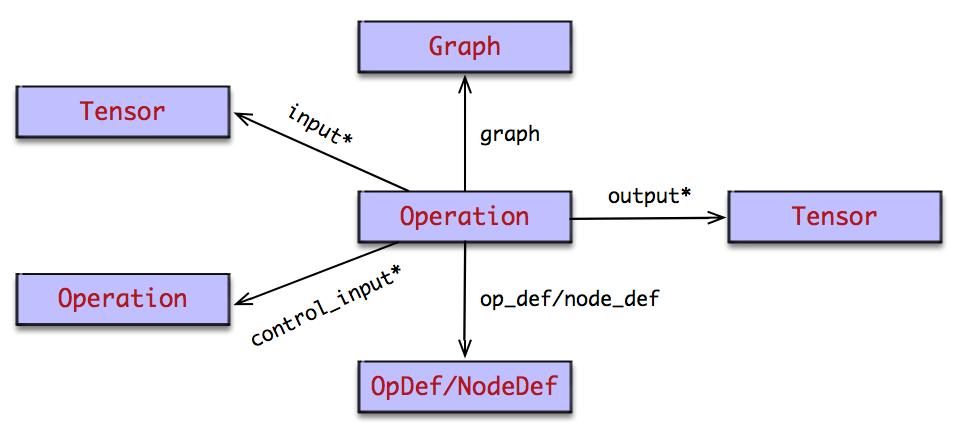
\includegraphics[width=0.9\textwidth]{figures/py-operation.png}
\caption{领域对象:Operation}
 \label{fig:py-operation}
\end{figure}

\subsection{Tensor}

一个\code{Tensor}表示\code{Operation}的某个输出的符号句柄,它并不持\code{Operation}输出的真实数据。可以通过\code{Session.run}计算得到\code{Tensor}所持有的真实数据。

如\refig{py-tensor}所示。\code{Tensor}是两个\code{Operation}数据交换的桥梁,它们之间构造了典型的「生产者-消费者」的关系。

\begin{figure}[!htbp]
\centering
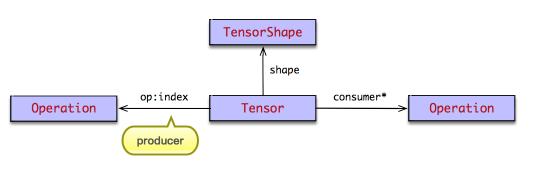
\includegraphics[width=0.9\textwidth]{figures/py-tensor.png}
\caption{领域对象:Tensor}
 \label{fig:py-tensor}
\end{figure}

其中,\code{Tensor}通过\ascii{op}持有扮演生产者角色的\code{Operation},并且使用\code{index}表示该\code{Tensor}在该\code{Operation}输出列表中的索引。也就是说,可以使用\code{op:index}的二元组信息在图中唯一标识一个\code{Tensor}实例。

此外,\code{Tensor}持有\code{Operation}的消费者列表。计算图以\code{Tensor}为边,构建\code{Operation}之间的数据连接,从而实现了整个计算图的数据依赖构建。

\subsubsection{生产者与消费者}

如\refig{py-tensor-producter-consumer}所示。上游\code{Operation}作为生产者,经过某种抽象计算,生产了一个\code{Tensor},并以此作为该上游\code{Operation}的输出之一,并使用\code{index}标识。

该\code{Tensor}被传递给下游\code{Operation},并作为下游\code{Operation}的输入,下游\code{Operation}充当该\code{Tensor}的消费者。

\begin{figure}[!htbp]
\centering
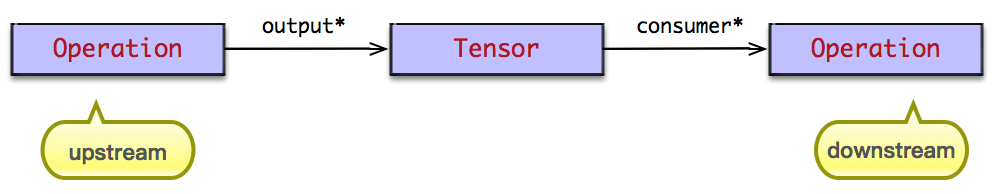
\includegraphics[width=0.9\textwidth]{figures/py-tensor-producter-consumer.png}
\caption{Tensor: 生产者-消费者关系}
 \label{fig:py-tensor-producter-consumer}
\end{figure}

\subsubsection{建立关联}

最后,参看\code{Operation}与\code{Tensor}的部分实现,很容易找两者「生产者-消费者」的关联关系。当\code{Tensor}列表作为输入流入\code{Operation}时,此时建立了下游\code{Operation}与输入的\code{Tensor}列表之间的消费关系。

\begin{leftbar}
\begin{python}
class Operation(object):
  def __init__(self, node_def, graph, inputs=None, output_types=None):
    # \_inputs as consumers
    self._inputs = list(inputs)
    for a in self._inputs:
      a._add_consumer(self)

    # self as producer
    self._output_types = output_types
    self._outputs = [Tensor(self, i, output_type)
                     for i, output_type in enumerate(output_types)]
\end{python}
\end{leftbar}


同样地,\code{Tensor}在构造函数中持有作为上游的的生产者\code{Operation},及其它在该\code{Operation}的\code{outputs}列表中的索引。此外,当调用\code{\_add\_consumer},将该下游\code{Operation}追加至消费者列表之中。

\begin{leftbar}
\begin{python}
class Tensor(_TensorLike):
  def __init__(self, op, value_index, dtype):    
    # Index of the OP's endpoint that produces this tensor.
    self._op = op
    self._value_index = value_index
    
    # List of operations that use this Tensor as input.  
    # We maintain this list to easily navigate a computation graph.
    self._consumers = []

  def _add_consumer(self, consumer):
    if not isinstance(consumer, Operation):
      raise TypeError("Consumer must be an Operation: %s" % consumer)
    self._consumers.append(consumer)
\end{python}
\end{leftbar}

\subsection{Graph}

如\refig{py-graph}所示。一个\code{Graph}对象将包含一系列\code{Operation}对象,表示计算单元的集合;同时,它间接持有一系列\code{Tensor}对象,表示数据单元的集合。

\begin{figure}[!htbp]
\centering
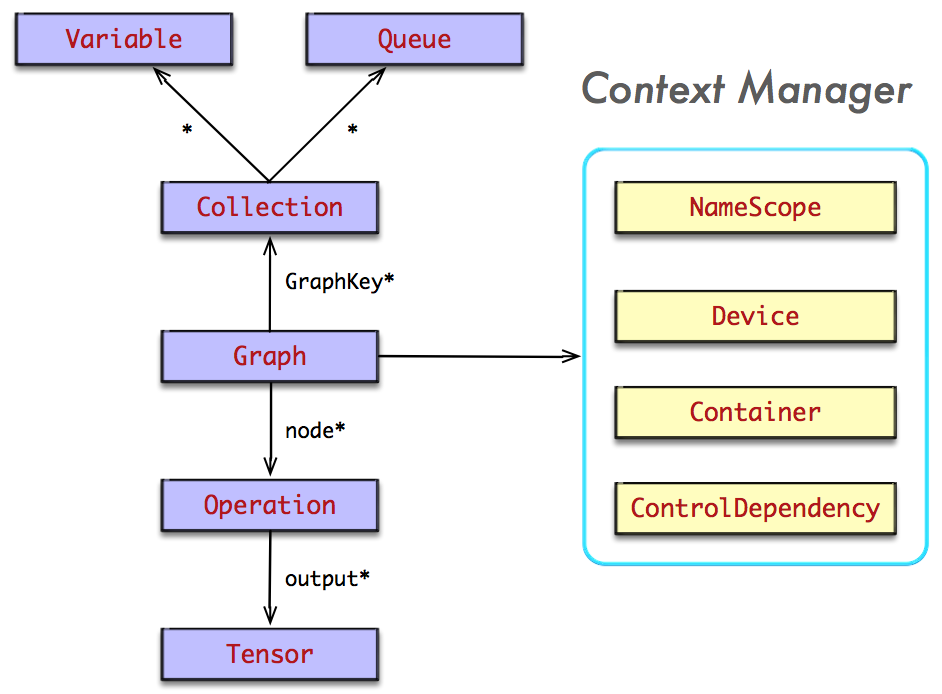
\includegraphics[width=0.9\textwidth]{figures/py-graph.png}
\caption{领域对象:Graph}
 \label{fig:py-graph}
\end{figure}

\subsection{图构造}

在计算图的构造期间,不执行任何\ascii{OP}的计算。简单地说,图的构造过程就是根据\ascii{OP}构造器完成\code{Operation}实例的构造。而在\code{Operation}实例的构造之前,需要实现完成\code{OpDef}与\code{NodeDef}的构造过程。

\subsubsection{OpDef仓库}

\code{OpDef}仓库在系统首次访问时,实现了\code{OpDef}的延迟加载和注册。也就是说,对于某中类型的\code{OpDef}仓库,\code{\_InitOpDefLibrary}模块首次导入时,扫描\code{op\_list\_ascii}表示的所有\ascii{OP},并将其转换为\ascii{Protobuf}格式的\code{OpList}实例,最终将其注册到\code{OpDefLibrary}实例之中。

例如,模块\code{gen\_array\_ops}是构建版本时自动生成的,它主要完成所有\code{array\_ops}类型的\code{OpDef}的定义,并自动注册到\code{OpDefLibrary}的仓库实例中,并提供按名查找\code{OpDef}的服务接口。

\begin{leftbar}
\begin{python}
_op_def_lib = _InitOpDefLibrary()

def _InitOpDefLibrary():
  op_list = _op_def_pb2.OpList()
  _text_format.Merge(_InitOpDefLibrary.op_list_ascii, op_list)   
  op_def_lib = _op_def_library.OpDefLibrary()
  op_def_lib.add_op_list(op_list)
  return op_def_lib

_InitOpDefLibrary.op_list_ascii = """op {
  name: "ZerosLike"
  input_arg {
    name: "x"
    type_attr: "T"
  }
  output_arg {
    name: "y"
    type_attr: "T"
  }
  attr {
    name: "T"
    type: "type"
  }
}
# ignore others
"""
\end{python}
\end{leftbar}

\subsubsection{工厂方法}

如\refig{py-op-factory-and-repo}所示。当\ascii{Client}使用\ascii{OP}构造器创建一个\code{Operation}实例时,将最终调用\code{Graph.create\_op}方法,将该\code{Operation}实例注册到该图实例中。

也就是说,一方面,\code{Graph}充当\code{Operation}的工厂,负责\code{Operation}的创建职责;另一方面,\code{Graph}充当\code{Operation}的仓库,负责\code{Operation}的存储,检索,转换等操作。

这个过程常称为计算图的构造。在计算图的构造期间,并不会触发运行时的\ascii{OP}运算,它仅仅描述计算节点之间的依赖关系,并构建\ascii{DAG}图,对整个计算过程做整体规划。

\begin{figure}[!htbp]
\centering
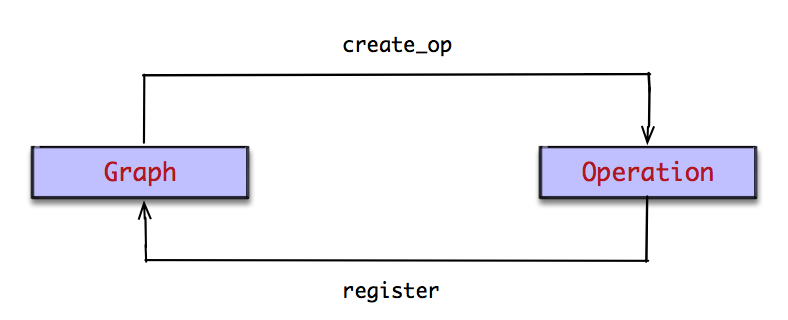
\includegraphics[width=0.9\textwidth]{figures/py-op-factory-and-repo.png}
\caption{Graph: OP工厂 + OP仓库}
 \label{fig:py-op-factory-and-repo}
\end{figure}

\subsubsection{OP构造器}

如\refig{py-op-constructor}所示。在图构造期,\ascii{Client}使用\code{tf.zeros\_like}构造一个名为\code{ZerosLike}的\ascii{OP},该\ascii{OP}拥有一个输入,输出一个全\ascii{0}的\ascii{Tensor};其中,\code{tf.zeros\_like}常称为\ascii{OP}构造器。

然后,\ascii{OP}构造器调用一段自动生成的代码,进而转调\code{OpDefLibrary.apply\_op}方法。

\begin{figure}[!htbp]
\centering
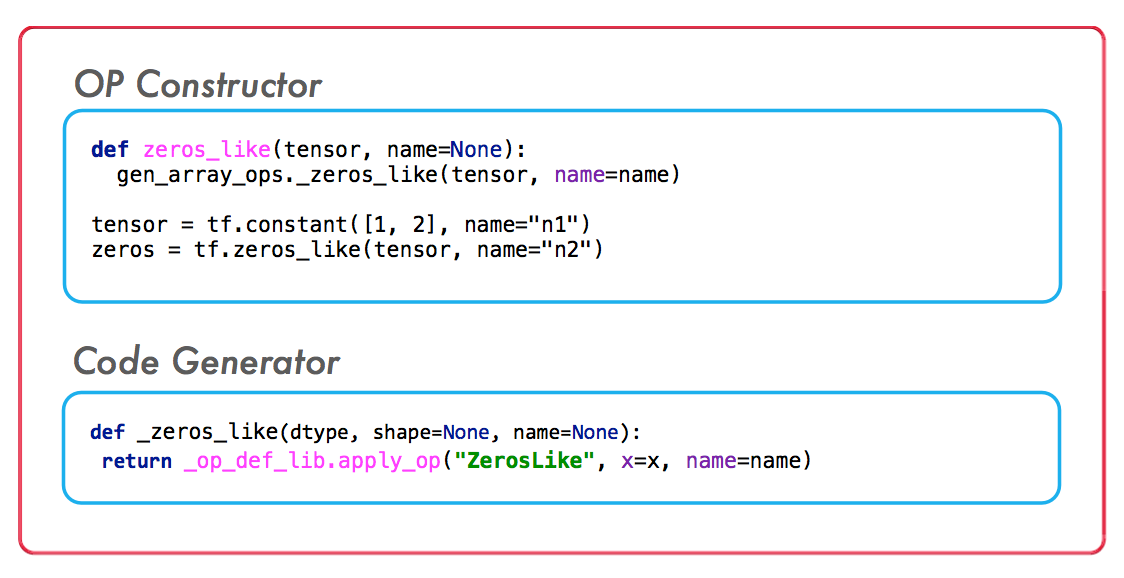
\includegraphics[width=0.9\textwidth]{figures/py-op-constructor.png}
\caption{OP构造器与代码生成器}
 \label{fig:py-op-constructor}
\end{figure}

\subsubsection{构造OpDef与NodeDef}

然后,如\refig{py-graph-create-op}所示。\code{OpDefLibrary}根据\ascii{OP}的名字从\code{OpDefLibrary}中,找到对应\code{OpDef}实例;最终,通过\code{Graph.create\_op}的工厂方法,创建\code{NodeDef}实例,进而创建\code{Operation}实例,将其自身注册到图实例中。

\begin{figure}[!htbp]
\centering
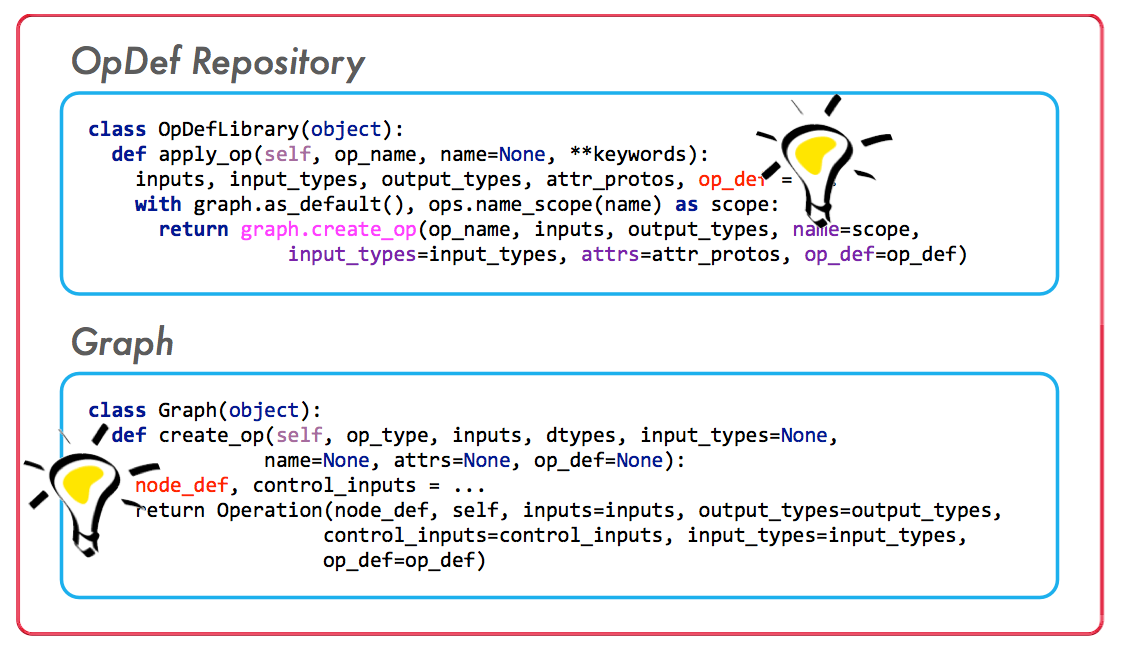
\includegraphics[width=0.9\textwidth]{figures/py-graph-create-op.png}
\caption{创建Operation实例: 创建OpDef, NodeDef实例}
 \label{fig:py-graph-create-op}
\end{figure}

\end{content}

\section{后端C++}

\begin{content}

在\ascii{C++}后端,计算图是\ascii{TensorFlow}领域模型的核心。

\subsection{边}

\code{Edge}持有前驱节点与后驱节点,从而实现了计算图的连接。一个节点可以拥有零条或多条输入边,与可以有零条或多条输出边。一般地,计算图中存在两类边:

\begin{enum}
  \eitem{普通边:用于承载数据(以\code{Tensor}表示),表示节点间“生产者-消费者”的数据依赖关系,常用实线表示;}
  \eitem{控制依赖:不承载数据,用于表示节点间的执行依赖关系,常用虚线表示。} 
\end{enum}

\subsubsection{两个标识}

\ascii{Edge}持有两个重要的索引:

\begin{enum}
  \eitem{\code{src\_output}:表示该边为「前驱节点」的第\code{src\_output}条输出边;}
  \eitem{\code{dst\_input}:表示该边为「后驱节点」的第\code{dst\_input}条输入边。} 
\end{enum}


\begin{figure}[!htbp]
\centering
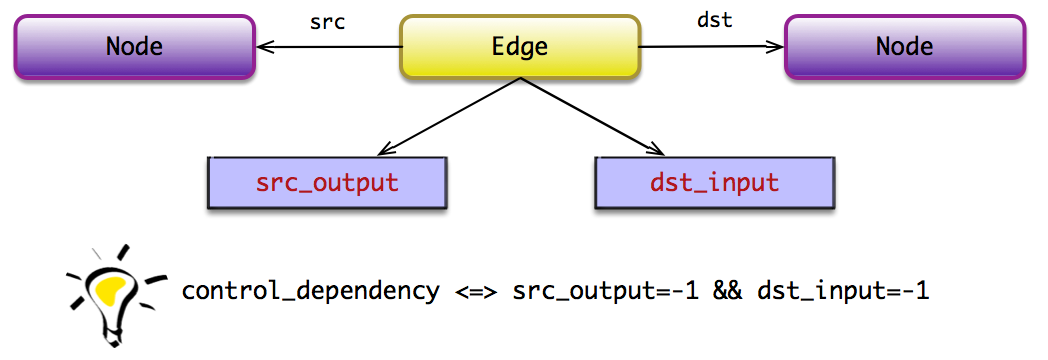
\includegraphics[width=0.9\textwidth]{figures/cc-edge-model.png}
\caption{领域对象:Edge}
 \label{fig:cc-edge-model}
\end{figure}

例如,存在两个前驱节点\code{s1, s2},都存在两条输出边;存在两个后驱节点\code{d1, d2},都存在两条输入边。

\begin{figure}[!htbp]
\centering
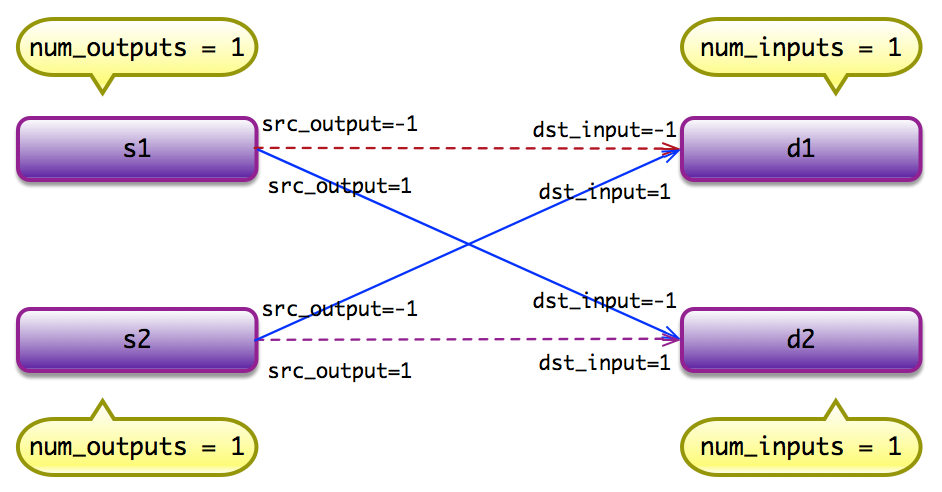
\includegraphics[width=0.9\textwidth]{figures/cc-edge-model-example.png}
\caption{边例子}
 \label{fig:cc-edge-model-example}
\end{figure}

\subsubsection{控制依赖}

对于控制依赖边,其\code{src\_output, dst\_input}都为\code{-1(Graph::kControlSlot)},暗喻控制依赖边不承载任何数据。

\begin{leftbar}
\begin{c++}
bool Edge::IsControlEdge() const {
   // or dst\_input\_ == Graph::kControlSlot;
   return src_output_ == Graph::kControlSlot;
}
\end{c++}
\end{leftbar}

\subsubsection{Tensor标识}

一般地,计算图的「普通边」承载\code{Tensor},并使用\code{TensorId}标识。\code{Tensor}标识由源节点的名字,及其所在边的\code{src\_output}唯一确定。

\begin{leftbar}
\begin{c++}
TensorId ::= node_name:src_output
\end{c++}
\end{leftbar}

缺省地,\code{src\_output}默认为\ascii{0};也就是说,\code{node\_name}与\code{node\_name:0}两者等价。特殊地,当\code{src\_output}等于\ascii{-1}时,表示该边为「控制依赖边」,\code{TensorId}可以标识为\code{\^node\_name},标识该边依赖于\code{node\_name}所在的节点。

\subsection{节点}

\code{Node}(节点)可以拥有零条或多条输入/输出的边,并使用\code{in\_edges, out\_edges}分别表示输入边和输出边的集合。另外,\code{Node}持有\code{NodeDef, OpDef}。其中,\code{NodeDef}包含设备分配信息,及其\ascii{OP}的属性值列表;\code{OpDef}持有\ascii{OP}的元数据,包括\ascii{OP}输入输出类型等信息。

\begin{figure}[!htbp]
\centering
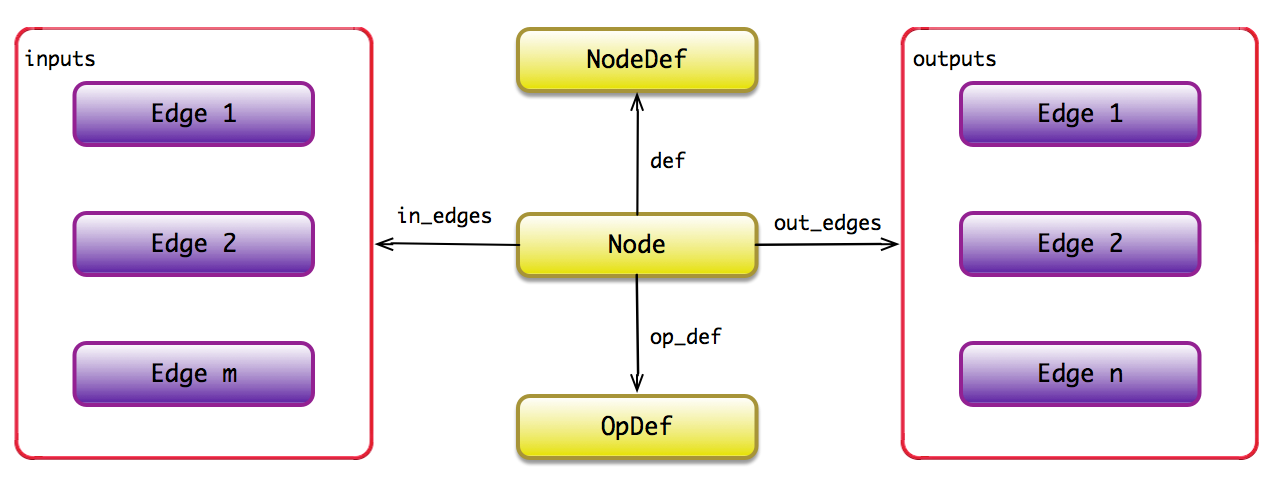
\includegraphics[width=0.9\textwidth]{figures/cc-node-model.png}
\caption{领域对象:Node}
 \label{fig:cc-node-model}
\end{figure}

\subsubsection{输入边}

在输入边的集合中,可以按照索引\code{(dst\_input)}线性查找。当节点输入的边比较多时,可能会成为性能的瓶颈。依次类推,按照索引\code{(src\_output)}查找输出边,算法类同。

\begin{leftbar}
\begin{c++}
Status Node::input_edge(int idx, const Edge** e) const {
  for (auto edge : in_edges()) {
    if (edge->dst_input() == idx) {
      *e = edge;
      return Status::OK();
    }
  }
  return errors::NotFound("not found input edge ", idx);
}
\end{c++}
\end{leftbar}

\subsubsection{前驱节点}

首先通过\code{idx}索引找到输入边,然后通过输入边找到前驱节点。依次类推,按照索引查找后驱节点,算法类同。

\begin{leftbar}
\begin{c++}
Status Node::input_node(int idx, const Node** n) const {
  const Edge* e = nullptr;
  TF_RETURN_IF_ERROR(input_edge(idx, &e));
  *n = e == nullptr ? nullptr : e->src();
  return Status::OK();
}
\end{c++}
\end{leftbar}

\subsection{图}

\code{Graph}(计算图)就是节点与边的集合。计算图是一个\ascii{DAG}图,计算图的执行过程将按照\ascii{DAG}的拓扑排序,依次启动\ascii{OP}的运算。其中,如果存在多个入度为\ascii{0}的节点,\ascii{TensorFlow}运行时可以实现并发,同时执行多个\ascii{OP}的运算,提高执行效率。

\begin{figure}[!htbp]
\centering

\includegraphics[width=0.9\textwidth]{figures/cc-graph-model.png}
\caption{领域模型:图}
 \label{fig:cc-graph-model}
\end{figure}

\subsubsection{空图}

计算图的初始状态,并非是一个空图。实现添加了两个特殊的节点:\code{Source}与\code{Sink}节点,分别表示\ascii{DAG}图的起始节点与终止节点。其中,\code{Source}的\code{id}为\ascii{0},\code{Sink}的\code{id}为\ascii{1};依次论断,普通\ascii{OP}节点的\ascii{id}将大于\ascii{1}。

\code{Source}与\code{Sink}之间,通过连接「控制依赖」的边,保证计算图的执行始于\code{Source}节点,终于\code{Sink}节点。它们之前的控制依赖边,其\code{src\_output, dst\_input}值都为\ascii{-1}。

\begin{figure}[!htbp]
\centering
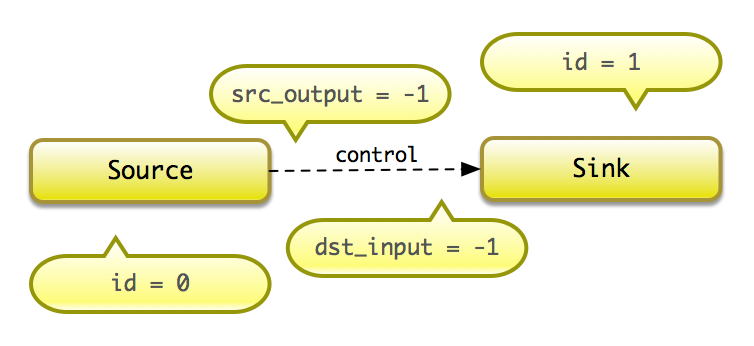
\includegraphics[width=0.9\textwidth]{figures/cc-empty-graph.png}
\caption{空图}
 \label{fig:cc-empty-graph}
\end{figure}

\code{Source}与\code{Sink}是两个内部实现保留的节点,其节点名称以下划线开头,分别使用\code{\_SOURCE}和\code{\_SINK}命名;并且,它们都是\code{NoOp},表示不执行任何计算。

\begin{leftbar}
\begin{c++}
Node* Graph::AddInternalNode(const char* name, int id) {
  NodeDef def;
  def.set_name(name);
  def.set_op("NoOp");

  Status status;
  Node* node = AddNode(def, &status);
  TF_CHECK_OK(status);
  CHECK_EQ(node->id(), id);
  return node;
}

Graph::Graph(const OpRegistryInterface* ops)
    : ops_(ops), arena_(8 << 10 /* 8kB */) {
  auto src  = AddInternalNode("_SOURCE", kSourceId);
  auto sink = AddInternalNode("_SINK",   kSinkId);
  AddControlEdge(src, sink);
}
\end{c++}
\end{leftbar}

习惯上,仅包含\code{Source}与\code{Sink}节点的计算图也常常称为空图。

\subsubsection{非空图}

在前端,用户使用\ascii{OP}构造器,将构造任意复杂度的计算图。对于运行时,实现将用户构造的计算图通过控制依赖的边与\code{Source/Sink}节点连接,保证计算图执行始于\code{Source}节点,终于\code{Sink}节点。

\begin{figure}[!htbp]
\centering
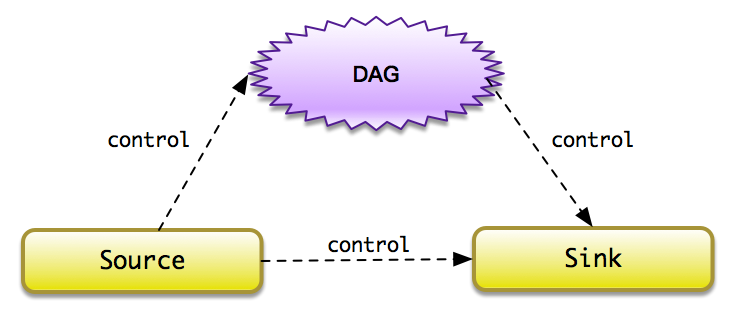
\includegraphics[width=0.9\textwidth]{figures/cc-non-empty-graph.png}
\caption{非空图}
 \label{fig:cc-non-empty-graph}
\end{figure}

\subsubsection{添加边}

计算图的构造过程非常简单,首先通过\code{Graph::AddNode}在图中放置节点,然后再通过\code{Graph::AddEdge}在图中放置边,实现节点之间的连接。

\begin{leftbar}
\begin{c++}
const Edge* Graph::AllocEdge() const {
  Edge* e = nullptr;
  if (free_edges_.empty()) {
    e = new (arena_.Alloc(sizeof(Edge))) Edge;
  } else {
    e = free_edges_.back();
    free_edges_.pop_back();
  }
  e->id_ = edges_.size();
  return e;
}

const Edge* Graph::AddEdge(Node* source, int x, Node* dest, int y) {
  auto e = AllocEdge();
  e->src_ = source;
  e->dst_ = dest;
  e->src_output_ = x;
  e->dst_input_ = y;

  CHECK(source->out_edges_.insert(e).second);
  CHECK(dest->in_edges_.insert(e).second);

  edges_.push_back(e);
  edge_set_.insert(e);
  return e;
}
\end{c++}
\end{leftbar}

\subsubsection{添加控制依赖边}

添加控制依赖边,则可以转发调用\code{Graph::AddEdge}实现;此时,\code{src\_output, dst\_input}都为\ascii{-1}。

\begin{leftbar}
\begin{c++}
const Edge* Graph::AddControlEdge(Node* src, Node* dst) {
  return AddEdge(src, kControlSlot, dst, kControlSlot);
}
\end{c++}
\end{leftbar}

\subsection{OpDef仓库}

同样地,\code{OpDef}仓库在\ascii{C++}系统\code{main}函数启动之前完成\code{OpDef}的加载和注册。它使用\ascii{REGISTER\_OP}宏完成\ascii{OpDef}的注册。

\begin{figure}[!htbp]
\centering
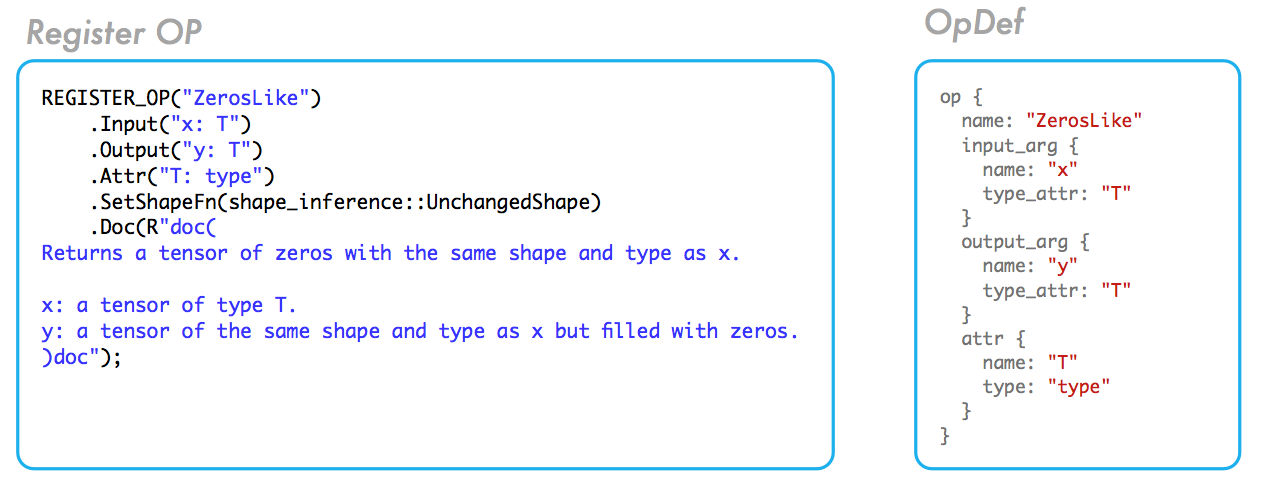
\includegraphics[width=0.9\textwidth]{figures/cc-op-repo.png}
\caption{OpDef注册:使用REGISTER\_OP}
 \label{fig:cc-op-repo}
\end{figure}

\end{content}

\section{图传递}

\begin{content}

\begin{figure}[!htbp]
\centering
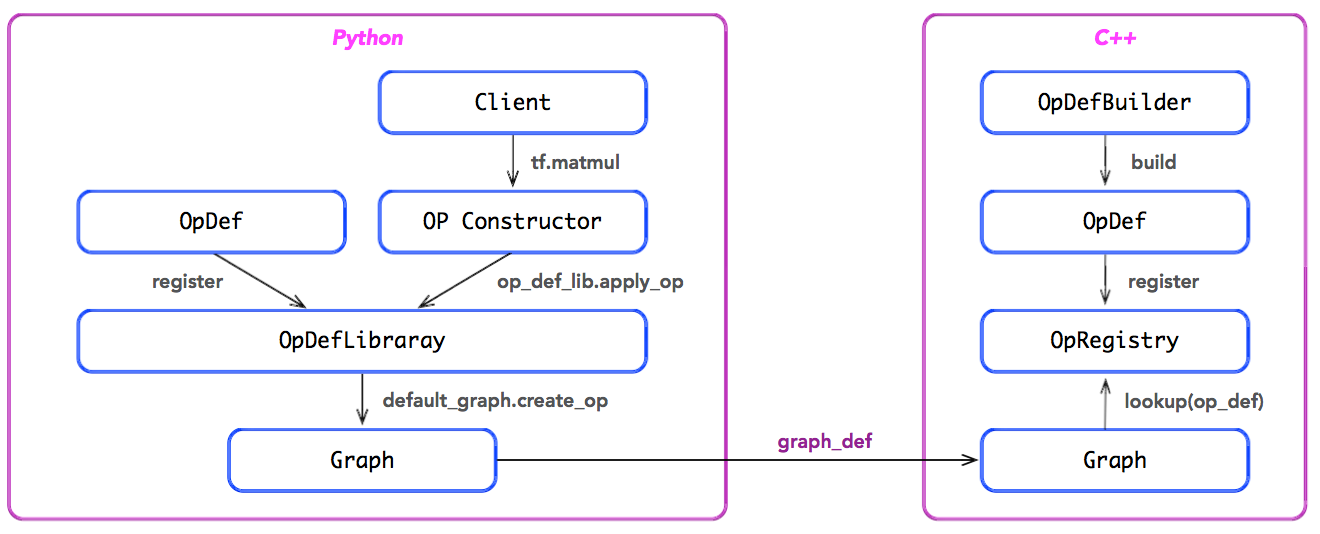
\includegraphics[width=0.9\textwidth]{figures/py-graph-creation.png}
\caption{图的序列化与反序列化}
 \label{fig:py-graph-creation}
\end{figure}

\end{content}

